\documentclass[a4paper,11pt]{report}
\usepackage[T1]{fontenc}
\usepackage[utf8]{inputenc}
\usepackage{lmodern}
\usepackage[francais]{babel}
\usepackage{graphicx}
\usepackage{array}

\title{Data wars }

\author{Guillaume LAROYENNE, Nathan PRETOT \\ Jeremy RENAUD, Tom SALVI, Pierre VALENZA}

\begin{document}

\maketitle
\tableofcontents

\chapter{Guide du joueur}

	\section{Inscription}
        Depuis le site vous trouverez en haut à droite de votre écran un bouton rouge "S'inscrire", cliquer et remplissez les champs correctement. 

	\section{Connexion}
        Depuis le site vous trouverez en haut à droite de votre écran un bouton bleu "Se connecter", cliquer et remplissez les champs correctement. 

	\section{Modifier mon deck}
       	Une fois connectez-vous êtes redirigés sur la gestion de votre deck, sinon cliquer sur le bouton mon deck dans la barre de navigation. 

	\begin{figure}[th]
		\begin{center}
		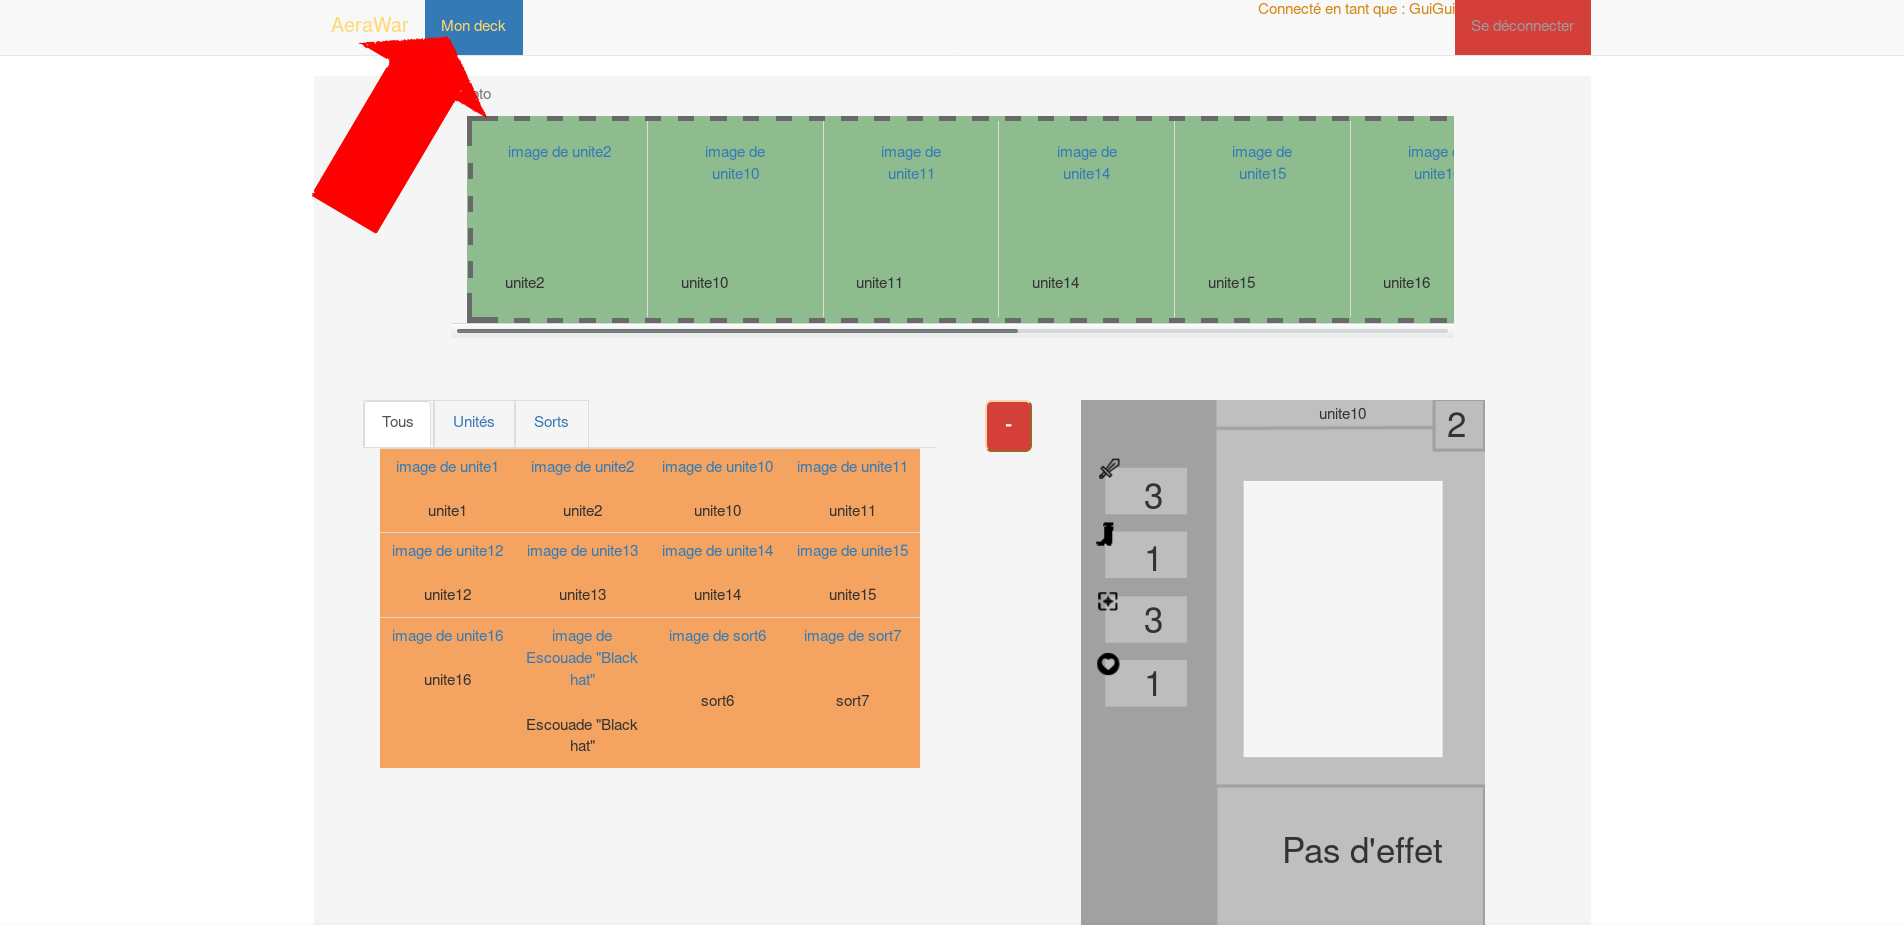
\includegraphics[scale=0.4]{Assets/go_deck.png}
      		\caption{Afficher son deck \textit{data wars}}
      		\label{fig1}
     		\end{center}
	\end{figure}

	Maintenant sélectionner une carte, peu importe si elle est présente dans votre deck. 	Vous allez remarquer que la carte c'est afficher sur la partie droite de l'écran.

	\begin{figure}[th]
		\begin{center}
		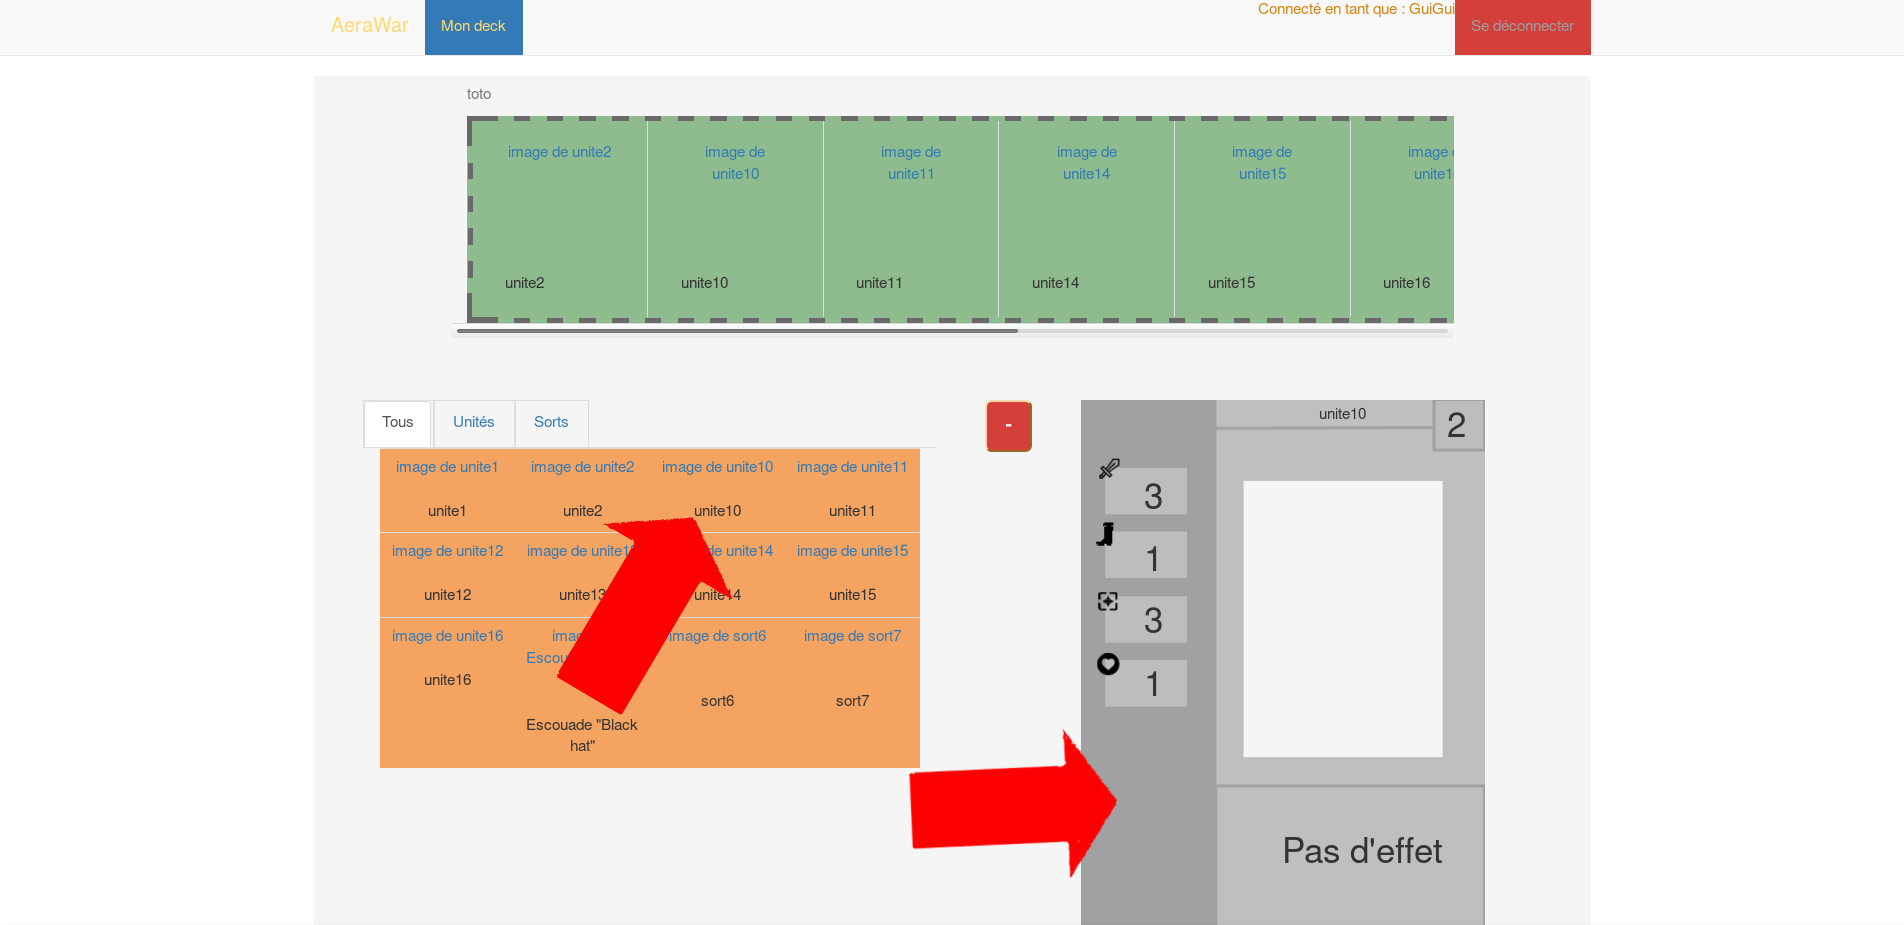
\includegraphics[scale=0.4]{Assets/carte_deck.png}
      		\caption{Selection d'une carte \textit{data wars}}
      		\label{fig2}
     		\end{center}
	\end{figure}

	À partir d'ici vous pouvez ajouter ou enlever la carte de votre deck.
\textit{RAPPEL : vous ne pouvez avoir plus de 15 cartes dans votre deck et une carte ne peut apparaitre plusieurs fois dans votre deck.}

	\begin{figure}[th]
		\begin{center}
		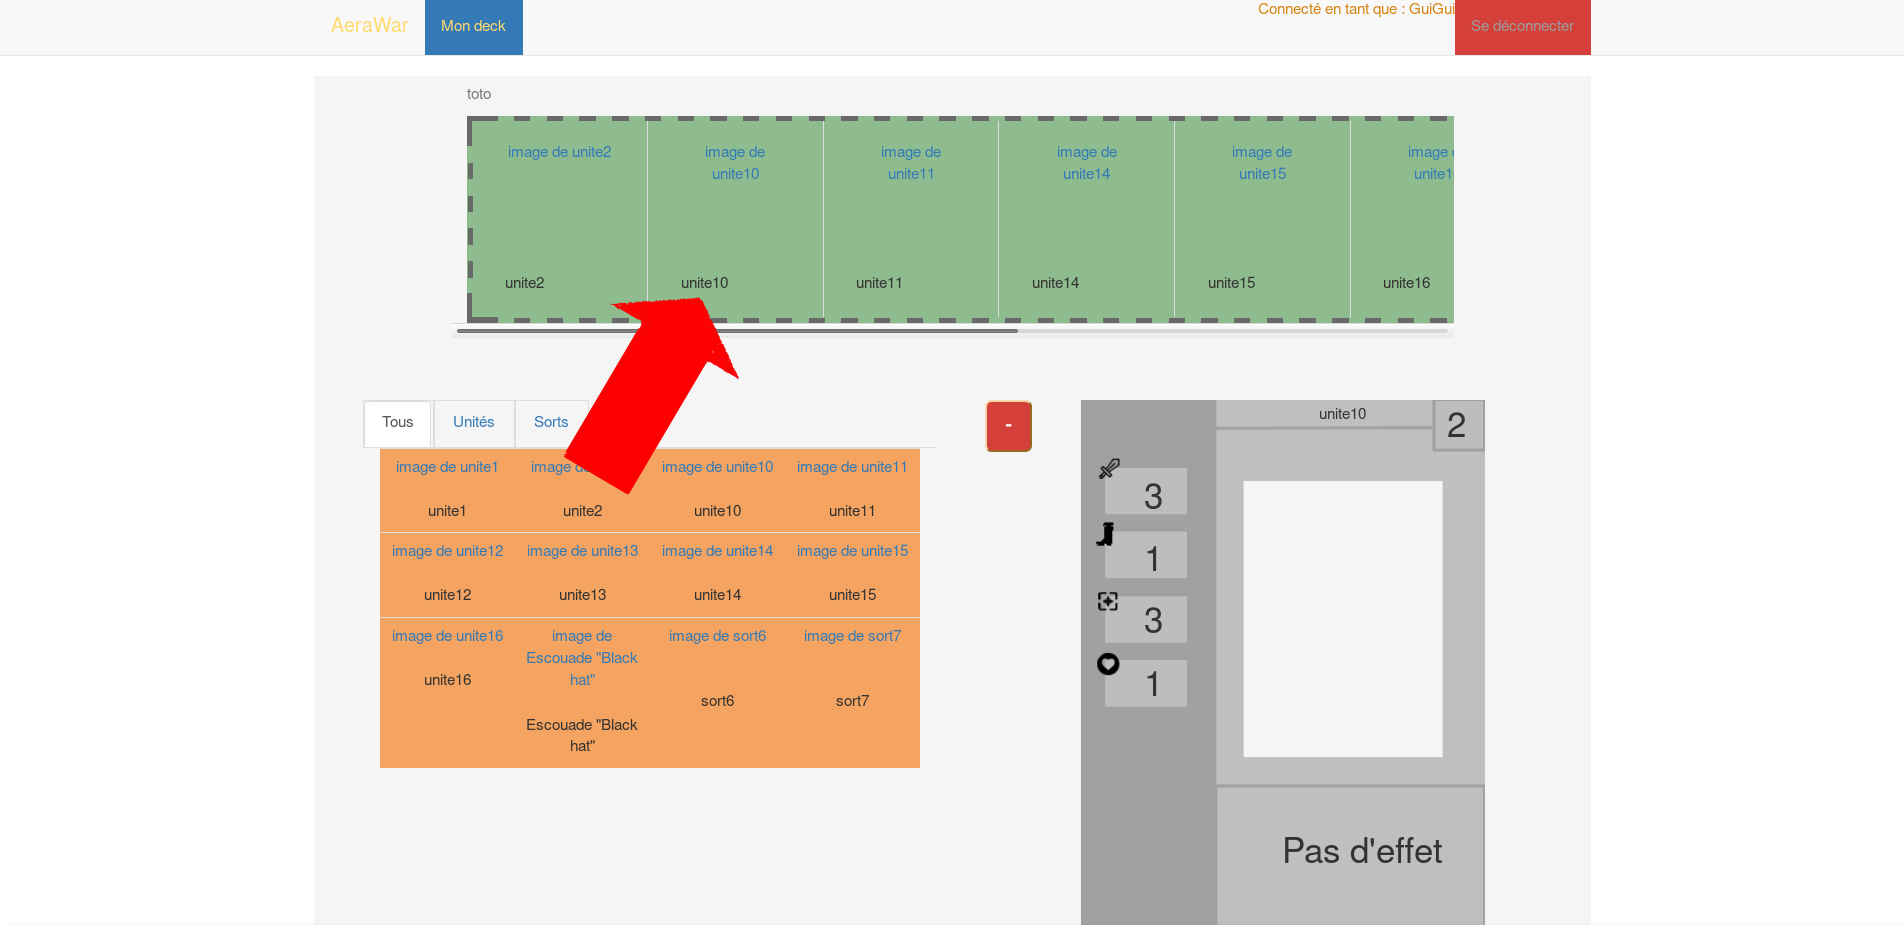
\includegraphics[scale=0.4]{Assets/add_deck.png}
      		\caption{Ajout d'une carte \textit{data wars}}
      		\label{fig2}
     		\end{center}
	\end{figure}

\chapter{Guide de l'administrateur}

	\section{Lister les cartes}
	Après votre connexion vous êtes automatiquement redirigé vers la liste des cartes. Vous pouvez aussi cliquer sur le bouton \textit{Voir les cartes} de votre barre de navigation.

	\section{Supprimer une carte}
	Lorsque vous êtes sur la liste des cartes, il suffit de cliquer sur la croix comme indiquer pour supprimer une carte.


	\section{Lister les clients}
	Vous pouvez cliquer sur le bouton \textit{Liste des clients} de votre barre de navigation pour accéder à la liste des clients.

	\section{Réinitialisé le deck d'un client}
	Lorsque vous êtes sur la liste des clients, cliquez sur la première option du client sélectionné.

	\section{Supprimer un clients}
	Lorsque vous êtes sur la liste des clients, cliquez sur la seconde option du client sélectionné.

	\section{Changer les droits du compte}
	Lorsque vous êtes sur la liste des clients, cliquez sur la troisième option du client sélectionné.

	\section{Lister et ajouter des effets}
	Vous pouvez cliquer sur le bouton \textit{Ajouter effets} de votre barre de navigation pour afficher la liste des effets. Pour ajouter un effet remplissez les champs textes.

	\section{Ajouter une carte}
		\subsection{Carte unité}
	Vous pouvez cliquer sur le bouton \textit{Ajout d'une carte unite} de votre barre de navigation, vous serez redirigé vers un formulaire à remplir.
		
		\subsection{Carte sort}
	Vous pouvez cliquer sur le bouton \textit{Ajout d'une carte sort} de votre barre de navigation, vous serez redirigé vers un formulaire à remplir.


        
\end{document}  

\grid
